\section{Remote shell with MPI}

\subsection{Protocol}

The graph below demonstrates the basic protocol for the client-server interaction that we implemented. The left column (rank X) represents the client while the right (rank Y) is the server. After a connection has been set up between two nodes, the program uses their rank X and Y to identify which side is the server and which side is the client.

Firstly, the server side sends the encrypted current directory to the client. After decryption, the user is able know which directory they are working on and create a command accordingly.

That command is then encrypted and sent to the server. After decryption, the server runs that command and sends the output back to the client.

The whole process above can be repeated as many times as desired until a kill signal is raised by the user. The connection between two nodes is cut afterwards.

\begin{center}
    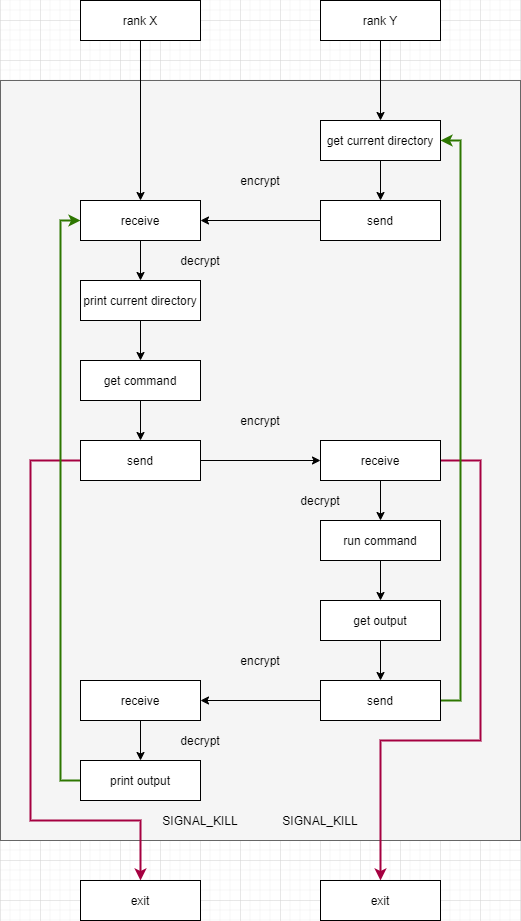
\includegraphics[scale=0.6]{images/client_server_protocol.png}
\end{center}

\subsection{Implementation}

\subsubsection{Required libraries}
Beside the mpi4py library to setup MPI connection, we need the subprocess and os library to execute shell commands and get their outputs.

We also import the written functions for data encryption and decryption in the security.py file from the above section.

\begin{minted}{python}
import mpi4py.MPI as MPI
import subprocess
import os

from security import import_key, encode_encrypt, decrypt_decode
   
\end{minted}

\subsubsection{MPI shell}

This function sets up a connection between two side. Inside of it, we create nested functions that define the behaviors of the client and the server according to the protocol. Rank 0 denotes the client and rank 1 denotes the server.

\begin{minted}{python}
def mpi_shell():
    """Setup a connection between two proccesses/two cores/two nodes/two clusters"""

    comm = MPI.COMM_WORLD
    rank = comm.Get_rank()

    if rank == 0:
        # client-like side
        # write mpi function to send and receive here
        
    elif rank == 1:
        # server-like side
        # write mpi function to send and receive here


if __name__ == '__main__':
    mpi_shell()

\end{minted}

\subsubsection{Client side}

\begin{minted}{python}
    if rank == 0:
        # client-like side

        # setup keys
        client_private_key = 'rank0/private.key.txt'
        server_public_key = 'rank1/public.key.txt'
        client_private_key, server_public_key = import_key(client_private_key, server_public_key)

        # enter client-server-like loop
        while True:
            cwd = decrypt_decode(comm.recv(source=1, tag=42), client_private_key)

            cmd = input(f'{cwd}#>')

            comm.send(encode_encrypt(cmd, server_public_key), dest=1, tag=42)

            output = decrypt_decode(comm.recv(source=1, tag=42), client_private_key)
            print(output)

\end{minted}

\subsubsection{Server side}

\begin{minted}{python}
    elif rank == 1:
        # server-like side

        # setup keys
        server_private_key = 'rank1/private.key.txt'
        client_public_key = 'rank0/public.key.txt'
        server_private_key, client_public_key = import_key(server_private_key, client_public_key)

        # enter server-client-like loop
        while True:
            cwd = os.getcwd()
            comm.send(encode_encrypt(cwd, client_public_key), dest=0, tag=42)

            cmd = decrypt_decode(comm.recv(source=0, tag=42), server_private_key)

            output = subprocess.getoutput(cmd)
            comm.send(encode_encrypt(output, client_public_key), dest=0, tag=42)
    
\end{minted}